\subsection{Decoders for Surface/Toric codes}
The Syndromes on the surface/toric code are a set of nodes and
faces on the code graph. The node ancilla syndromes correspond to
Z errors, while the face ancilla syndromes correspond to X errors.
Since neighboring errors will trigger an ancilla that is between 
both errors twice, a chain of errors will only appear as two ancilla
syndrome bits being flipped at its borders.
The task of a decoding scheme for a surface/toric code is thus to
find the shortest paths between node pairs/face pairs, since the most likely
chain of errors to occur given a $<50\%$ physical error rate is the 
shortest one.\\
In practice, decoders for surface/toric codes only need to be able to
match nodes, since the matching of faces is just matching nodes on the 
dual graphs and the resulting data qubit errors can just be joined
(i.e. if an edge is found to have an error on both the X graph as well as the
dual Z graph, we know a Y error has occurred on that edge/data-qubit).
An example of a distance 5 surface code with two Z errors, one X error and
one Y error is shown in figure \ref{fig: surface_code}.
As with the ringcode, the decoding problem can be seen as either the
solution of equation \ref{eq: pcm} for a minimum weight $\vec{v}_{error}$
or as a graph matching problem.
\subsubsection{MWPM decoding}
The \emph{Minimum-Weight Perfect Matching} algorithm is a variant of 
Dijkstra's algorithm that can be used to find the shortest vector of edges
that are bounded by the input syndrome nodes.
The algorithm is as follows:
\begin{enumerate}
    \item Find a set of unmatched nodes that can be reached from the 
    Matching\footnote{In graph theory, a matching is a subset of graph
    edges such that no two edges share a common vertex. The Goal of the MWPM
    algorithm is to find a Matching with minimum weight, i.e. a shortest vector of
    edges} by alternating between matched and unmatched edges. 
    Call these nodes "augmenting nodes".
    \item Find an augmenting path starting from each augmenting node,
    i.e. a path that starts and ends with an unmatched node, and
    alternates between matched and unmatched edges. 
    \item If such a path is found, flip all edges along it from matched
    to unmatched, and vice versa.
    \item Repeat until no augmenting path is found.
\end{enumerate}

This decoding scheme has the advantage of being guaranteed
to find a global optimum of decoding edge paths, i.e. it always finds the shortest vector
of edges that are bounded by the syndrome nodes.
Under the assumption of high error rates and/or large decoding 
graphs, this scheme also requires significantly less
computational memory overhead than the union-find scheme
\cite{MWPMDecoder}.
\subsubsection{Union-Find decoder}
\begin{enumerate}
    \item Initialize a cluster set for each syndrome node
    \item Grow each cluster by one edge in each direction
    \item Merge all clusters that share a node
    \item For all clusters with an even amount of syndrome nodes,
    perform MWPM within that cluster. Pop the found error edges from
    the graph.
    \item Repeat until all clusters are merged/discarded.
\end{enumerate}
While the union-find decoder is faster for small to medium
sized graphs and relatively simple to implement,
 it is not guaranteed to find a global optimum
and its performance degrades significantly for large
graphs and high error rates \cite{UFDecoder}.
For this reason, a MWPM algorithm was chosen for decoding the toric
subgraphs of the color code in our lifting decoder thresholding
in Chapter \ref{sec: lifting}.

\subsection{Color code decoders}
Unlike the surface and toric codes, in the color code the 
data qubits sit on the graphs nodes, and the ancillas on the 
graphs faces. Decoding the color code entails matching 
three differently colored faces to its enclosed nodes.
This is a significantly more challenging task than
decoding the 2D-codes, since three-colored graph matching is a confirmed
NP-hard problem. (reference delfosse paper)
\subsubsection{Lookup table decoding}
A lookup table decoder works by generating the 
syndromes for the entire set of possible input errors, thus creating a 
table holding possible errors responsible for each possible syndrome.
The decoding then consists of merely assuming the minimum weight
error that leads to the known syndrome, since given low physical 
error rate, the least amount of errors leading to an error is the most
probable event.

This decoding scheme is particularly useful for small codes, as well 
as non-topological (random) LDPC (Low-Density-Parity-Check) codes.
A big issue with this decoding scheme is that generating lookup tables is
extremely computationally expensive $(O(2^n))$. This renders it practically
unfeasible to generate lookup tables for codes with a larger number
of total data qubits.

\begin{figure}[h!]
	\begin{center}
	\captionsetup{justification=centering,margin=2cm}
	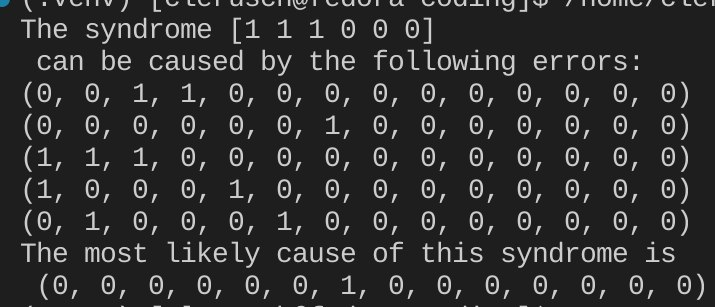
\includegraphics[scale=0.7]{./img/figures/X7errorlookup.png}\\
	\caption{Lookup table for an X error on the central qubit of
    a Steane code (qubit 7), generating code can be found in Appendix
    \ref{App: lookup_table}}
        
	\label{fig: lookup_table}
	\end{center}
\end{figure}

In figure \ref{fig: lookup_table} is an example of the lookup table result for
an X error on qubit 7 (the central qubit) on the Steane code. 
The resulting syndrome is (1,1,1,0,0,0), with the first three
bits indicating the steane code faces X reaction, and the second three bits
indicating the Steane code faces Z reaction. 
The lookup table will return a set of many possible errors resulting in 
that syndrome, but simply choosing the one with the least number of errors 
(minimum weight) gives the correct error prediction.

Since this is not a distance-scalable code, only a $pseudo$-threshold can
be found here, i.e. the crossing point to worse performance than unencoded
information. As can be seen in figure \ref{fig: steane_threshold}, the
pseudo-threshold is somehow very bad. I do not know why.

\begin{figure}[h!]
	\begin{center}
	\captionsetup{justification=centering,margin=2cm}
	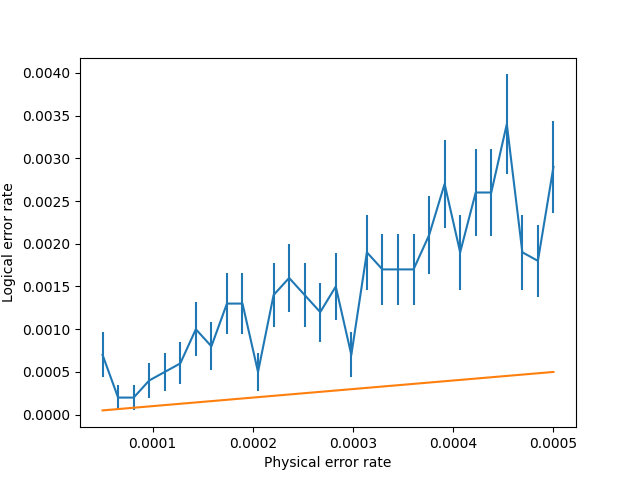
\includegraphics[scale=0.7]{./img/figures/thresholds/steaneLookupThreshold.png}\\
	\caption{Lookup table pseudo threshold for the Steane code, generating code can be found in Appendix
    \ref{App: steane_thresholding}}
        
	\label{fig: steane_threshold}
	\end{center}
\end{figure}
\newpage
\subsubsection{Lifting decoder}\label{sec: lifting}
The Lifting decoder works as follows:
\begin{itemize}
    \item Create dual of Tanner graph
    \item Generate single-edge-colored subgraphs of the dual
    \item Decode subgraphs using MWPM/Union-Find
    \item Unify all edges from subgraph corrections
    \item Find all shortest-length loops on this union
    \item NOLIFTING CASE ????
    \item All nodes bounded by the faces that are elements of the shortest-length loop sets
    are error nodes. 
\end{itemize}
By sub-tiling
the graph into smaller subgraphs, we can reduce the problem of decoding
e.g. a honeycomb lattice toric color code to a set of
MWPM-decodable toric graphs that merely need to be "lifted" into a 
combination of subgraph decodings to decode the original color code
graph \cite{delfosse}. 
\begin{figure}[h!]
    \centering
    \subfigure[Original toric honeycomb lattice color code. Errors are marked yellow, \
    face colors are implied by opposing colors wrapping them.]{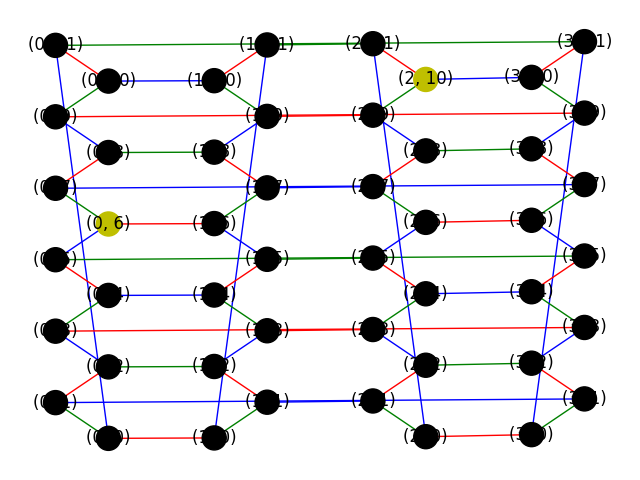
\includegraphics[width=0.4\textwidth]{img/figures/original.png}}\hfill
    \subfigure[Dual of color code lattice. Nodes are faces on the original lattice\
    yellow marked nodes represent syndromes.]{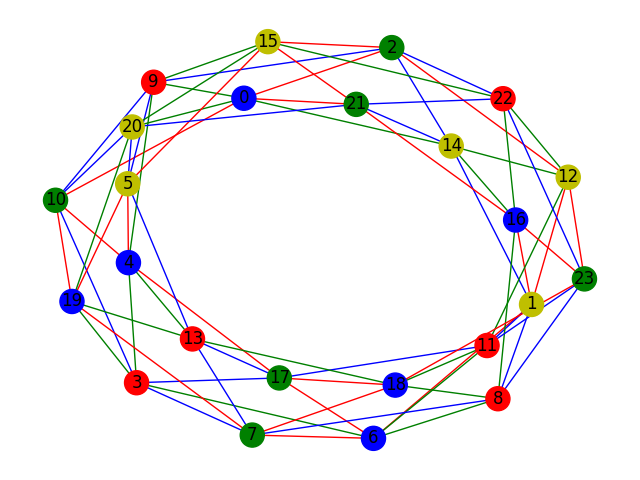
\includegraphics[width=0.4\textwidth]{img/figures/dual.png}}\hfill
    \subfigure[Red subgraph to be decoded via MWPM]{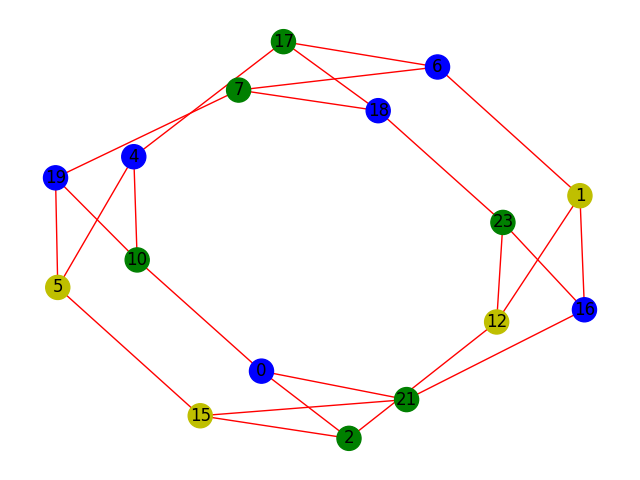
\includegraphics[width=0.4\textwidth]{img/figures/0.png}}\hfill
    \subfigure[Correct error prediction output for single distributed error nodes.]{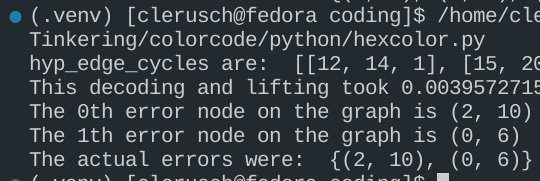
\includegraphics[width=0.4\textwidth]{img/figures/correctLiftingPred.png}}
    \caption{Steps in the lifting decoder. Generating code can be found in\ref{App: lifting}\
    and the entire git repository can be found in \cite{clemens}}
    \label{fig: lifting}
\end{figure}
This decoding is not optimal, as it does not take into account the other two colored
subgraphs when computing an MWPM edge prediction.
The polynomial time complexity of the lifting decoder does not
violate the NP-hardness of the 3-color matching problem, since the 
lifting procedure does not provide an optimal solution.
A graphical depiction of the steps of the lifting decoder is shown in
figure \ref{fig: lifting}.
\newpage